\chapter{Introduction to Boosting \label{chapter:boosting}}

Random forests (Chapter~\ref{chapter:randomforests}) are one approach to ensemble learning. Today we will examine another approach, \textbf{boosting}, that relies on a completely different set of ideas. The first practical boosting algorithm, AdaBoost, was invented in 1995 by Freund and Schapire. However, boosting is a general approach to choosing a set of weak learners that, together, create a strong learner. Since the same idea has spawned many different approaches, boosting is referred to as a \textbf{meta-algorithm}. 

%%%%%%%%%%%%%%%%%%%%%%%%%%%%%%%%%%%%%%%%%%%%%%%%%%%%%%%%%%%%%%%%%%%%%%%%%%%%%%%%%%%%%%%%

\section{AdaBoost}

Assume we are trying to solve a supervised learning problem. As usual, our data look like this:
$$\{ (x^{(1)}, y^{(1)}),  \dots, (x^{(n)}, y^{(n)}) \}$$

\noindent where the $x^{(i)}$ are feature vectors of length $p$. For now, we will assume that the outcome, $Y$, is binary (so this is a binary classification problem -- see Chapter~\ref{chapter:classification}). We'll make one small notational change from earlier chapters. Instead of $Y \in \{0, 1\}$, we'll say $Y \in \{-1, 1\}$. The fact that the positive and negative training examples have opposite sign will help us write the algorithm more concisely. 

The basic strategy behind AdaBoost is to build classifiers in series while maintaining a set of weights for the different training examples. The weights change with each subsequent classifier, increasing if previous classifiers have made incorrect predictions and decreasing if previous classifiers were correct. In this way, the importance of difficult-to-classify training examples increases, leading us to prefer future classifiers that successfully predict these examples. 

Here is the algorithm:

\begin{enumerate}
\item Initialize the observation weights to $w_i^{(1)} = \frac{1}{N}$ for $i = 1, \dots, N$.
\item For $m = 1, \dots, M$:
    \begin{enumerate}
    \item[(a)] Select a classifier, $G_m(x)$, that minimizes the weighted training error according to the current set of weights, $w_i^{(m)}$. Depending on the algorithm, it may be possible to train a single classifier on the weighted training set; in other cases, one may need to select the best-performing classifier from among a predefined set. 
    \item[(b)] Compute
    $$ \text{err}_m = \frac{\sum_{i=1}^N w_i^{(m)} \cdot \mathcal{I}(y^{(i)} \neq G_m (x^{(i)}))}{\sum_{i=1}^N w_i^{(m)}} $$
    \item[(c)] Compute voting weight for classifier $m$:
    $$ \alpha_m = \log \left( \frac{1 - \text{err}_m}{\text{err}_m} \right) $$
    \item[(d)] Set 
    $$ w_i^{(m+1)} \coloneqq w_i^{(m)} \cdot \text{exp} \left[ \alpha_m \cdot \mathcal{I}(y^{(i)} \neq G_m (x^{(i)})) \right] $$
    for $i = 1, \dots, N$. 
    \end{enumerate}
\item Output 
$$G(x) = \text{sign} \left[ \sum_{m=1}^M \alpha_m G_m(x) \right]$$
\end{enumerate}

The output definition in step~$3$ is really the key to the whole thing. Your goal is to construct a set of classifiers whose votes will be added together to produce an overall decision. AdaBoost provides one possible set of instructions for how to choose/build the individual classifiers, $G_m(x)$, and how to weight their votes. 

%%%%%%%%%%%%%%%%%%%%%%%%%%%%%%%%%%%%%%%%%%%%%%%%%%%%%%%%%%%%%%%%%%%%%%%%%%%%%%%%%%%%%%%%

\section{Visualizing the Steps of AdaBoost}

We will now train AdaBoost on the happiness dataset from Section~\ref{section:happiness}. Here is the dataset, using the new notation for $Y$. The astute observer will notice that we've added a fourth covariate, $X_4$ (whether or not the person has a pet). The reason is that subjects $5$ and $10$ are exactly the same otherwise, so we can never get perfect separation using the original dataset.

{\small
\begin{center}
\begin{tabular}{cccccc}
\toprule
Subject ID & friends $(X_1)$ & money $(X_2)$ & free time $(X_3)$ & pet $(X_4)$ & happy $(Y)$ \\
\midrule
1 & 1 & 1 & 0 & 0 & -1 \\
2 & 1 & 1 & 1 & 0 & -1 \\
3 & 0 & 1 & 1 & 0 & -1 \\
4 & 0 & 0 & 0 & 0 & -1 \\
5 & 1 & 0 & 0 & 0 & -1 \\
6 & 0 & 0 & 0 & 0 & -1 \\
\midrule
7 & 1 & 2 & 1 & 0 & 1 \\
8 & 1 & 0 & 1 & 0 & 1 \\
9 & 0 & 0 & 1 & 1 & 1 \\
10 & 1 & 0 & 0 & 1 & 1 \\
\bottomrule
\end{tabular}

\begin{align*}
	X_1 &= \left\{ \begin{array}{cl} 0 & \text{no friends} \\ 1 & \text{friends} \end{array} \right.
	&
	X_2 &= \left\{ \begin{array}{cl} 0 & \text{poor} \\ 1 & \text{enough money} \\ 2 & \text{rich} \end{array} \right. \\
	X_3 &= \left\{ \begin{array}{cl} 0 & \text{no free time} \\ 1 & \text{some free time} \end{array} \right.
	&
	X_4 &= \left\{ \begin{array}{cl} 0 & \text{no pet} \\ 1 & \text{has a pet} \end{array} \right.
\end{align*}
\end{center}
}
\vspace{3mm}

\noindent Now, let's go through the process of applying AdaBoost to this dataset, step by step. 

\begin{enumerate}
\item[(a)] Initialize the observation weights for the training data. (Make them uniform.)
\begin{center}
\begin{tabular}{p{0.45\textwidth}p{0.45\textwidth}}
$w_1^{(1)} = $ \hfill & $w_6^{(1)} = $ \hfill \\
$w_2^{(1)} = $ \hfill & $w_7^{(1)} = $ \hfill \\
$w_3^{(1)} = $ \hfill & $w_8^{(1)} = $ \hfill \\
$w_4^{(1)} = $ \hfill & $w_9^{(1)} = $ \hfill \\
$w_5^{(1)} = $ \hfill & $w_{10}^{(1)} = $ \hfill \\
\end{tabular}
\end{center}

\item[(b)] We will now grow a decision tree on this dataset, $G_1(x)$, using these weights. We'll use the \texttt{rpart} package in R, just as in Section~\ref{section:happiness}. Here is the first tree.

\begin{center}
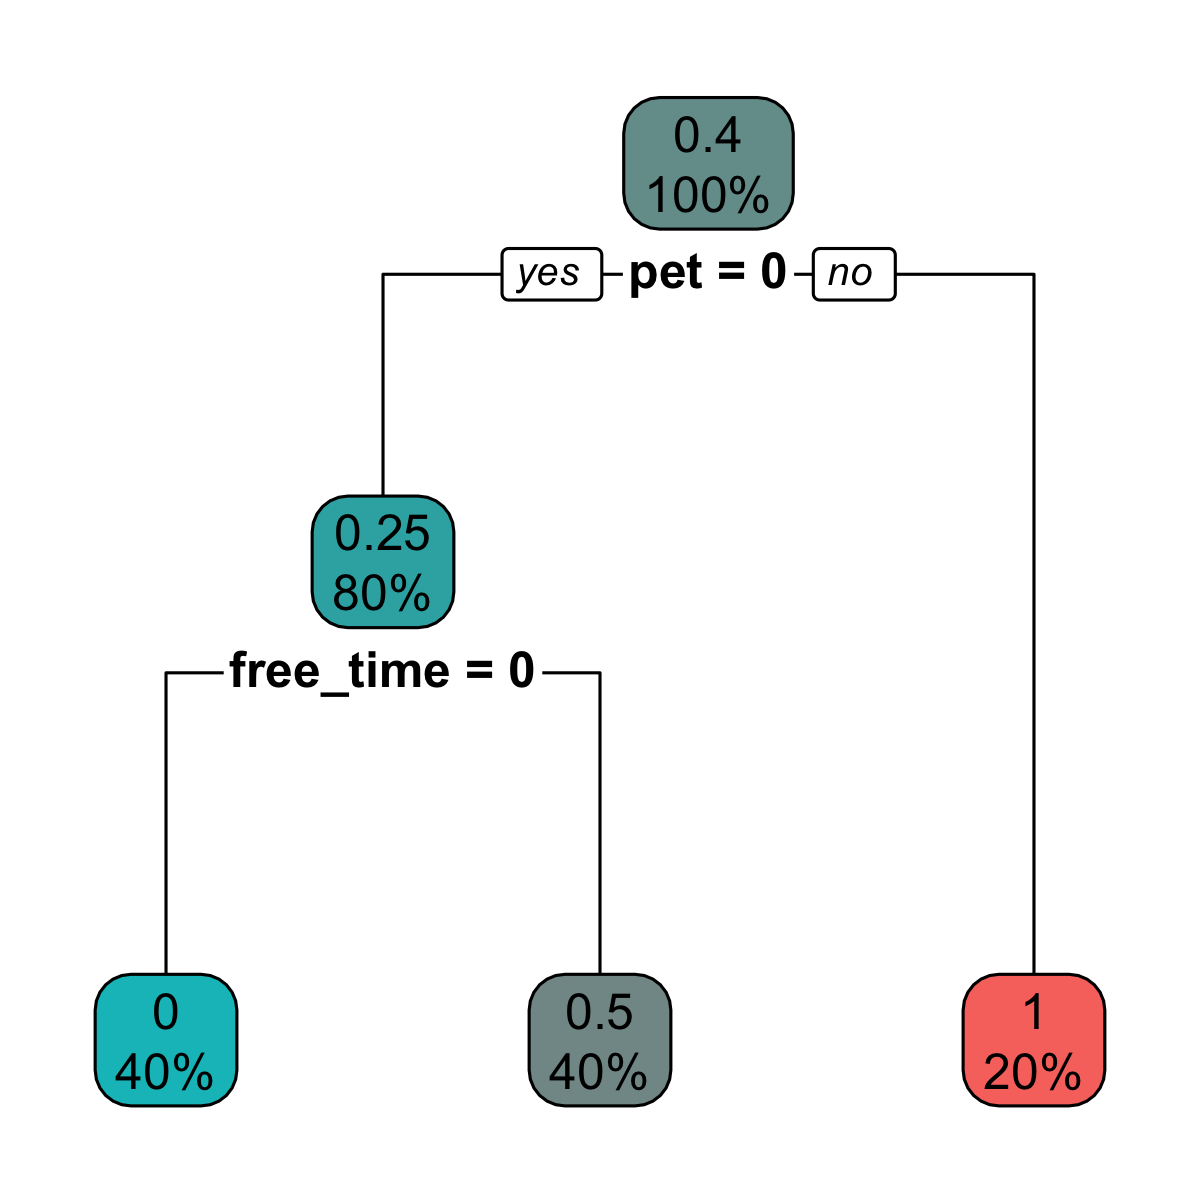
\includegraphics[width=0.6\textwidth]{img/happiness-boosting-tree-1.png}
\end{center}

\noindent Here are the predictions for this tree, along with the current weights.

{\small
\begin{center}
\begin{tabular}{cccc}
\toprule
Datapoint ID & $w_i^{(1)}$ & happy $(Y)$ & $G_1(x)$ \\
\midrule
1 & 0.1 & -1 & -1 \\
2 & 0.1 & -1 & -1 \\
3 & 0.1 & -1 & -1 \\
4 & 0.1 & -1 & -1 \\
5 & 0.1 & -1 & -1 \\
6 & 0.1 & -1 & -1 \\
\midrule
7 & 0.1 & 1 & -1 \\
8 & 0.1 & 1 & -1 \\
9 & 0.1 & 1 & 1 \\
10 & 0.1 & 1 & 1 \\
\bottomrule
\end{tabular}
\end{center}
}

\noindent Compute the misclassification error of this tree, $\text{err}_1$. Compare this tree to the one we constructed by hand in Chapter~\ref{chapter:decisiontrees}.

$$ \text{err}_1 = \qquad \qquad \qquad $$
\vspace{3mm}

\item[(c)] Based on how $G_1(x)$ performs, calculate $\alpha_1$, its voting weight.
$$ \alpha_1 = \qquad \qquad \qquad $$

\item[(d)] Re-weight the observation weights for the training examples.
\begin{center}
\begin{tabular}{p{0.45\textwidth}p{0.45\textwidth}}
$w_1^{(2)} = $ \hfill & $w_6^{(2)} = $ \hfill \\
$w_2^{(2)} = $ \hfill & $w_7^{(2)} = $ \hfill \\
$w_3^{(2)} = $ \hfill & $w_8^{(2)} = $ \hfill \\
$w_4^{(2)} = $ \hfill & $w_9^{(2)} = $ \hfill \\
$w_5^{(2)} = $ \hfill & $w_{10}^{(2)} = $ \hfill \\
\end{tabular}
\end{center}

\item[(e)] Now we grow another decision tree, $G_2(x)$, using these new weights as inputs to the \texttt{rpart} package.

\begin{center}
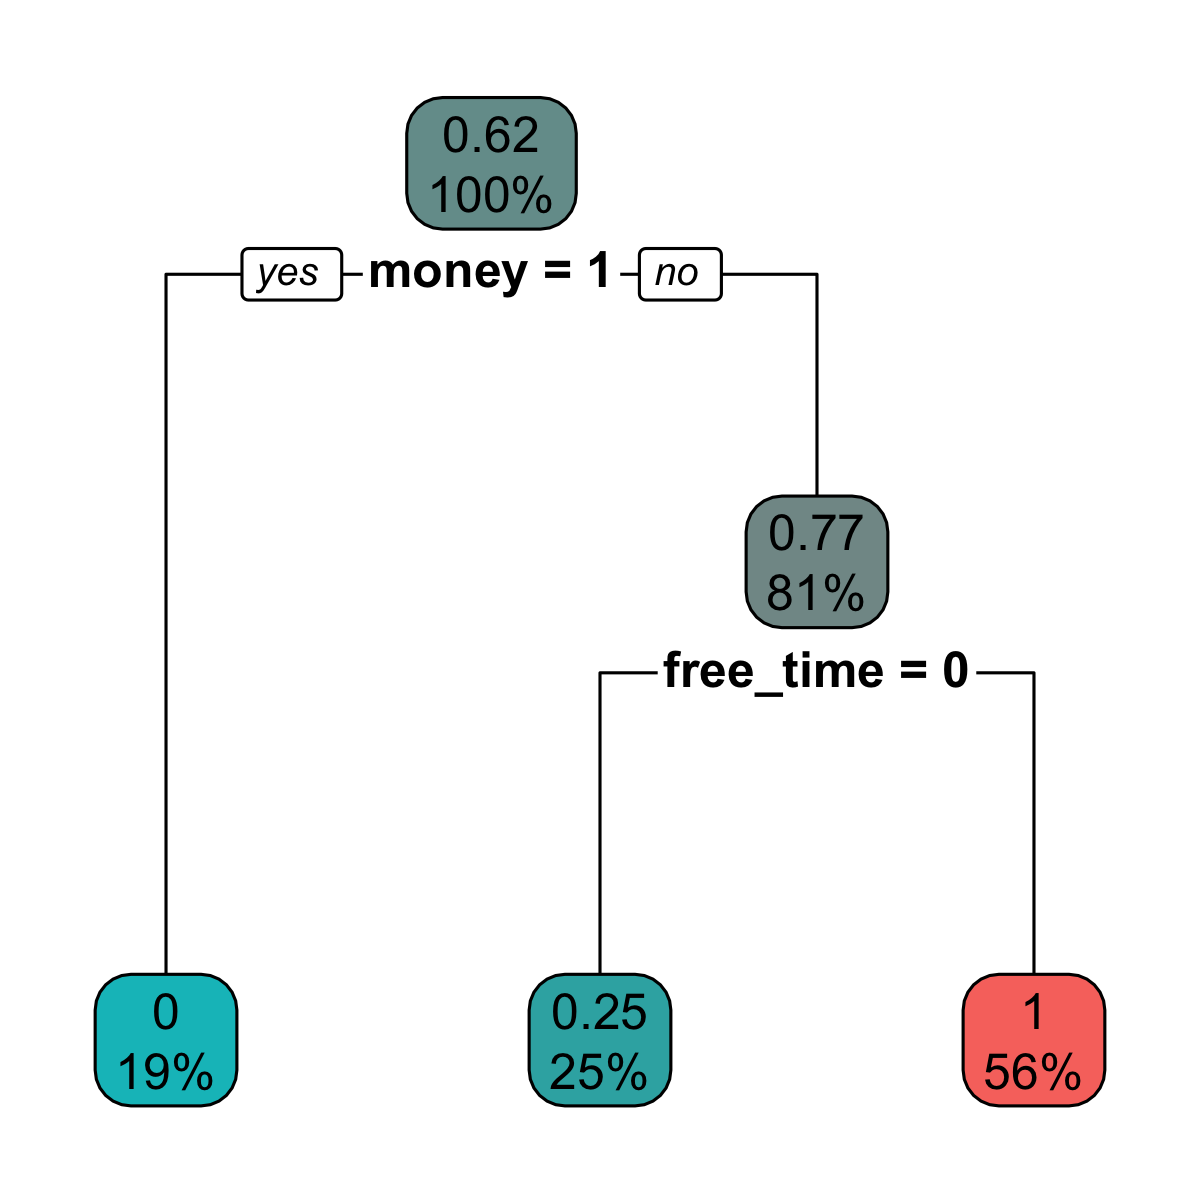
\includegraphics[width=0.6\textwidth]{img/happiness-boosting-tree-2.png}
\end{center}

Here are the predictions for this tree, along with the current weights.

{\small
\begin{center}
\begin{tabular}{cccc}
\toprule
Datapoint ID & $w_i^{(2)}$ & happy $(Y)$ & $G_2(x)$ \\
\midrule
1 & 0.1 & -1 & -1 \\
2 & 0.1 & -1 & -1 \\
3 & 0.1 & -1 & -1 \\
4 & 0.1 & -1 & -1 \\
5 & 0.1 & -1 & -1 \\
6 & 0.1 & -1 & -1 \\
\midrule
7 & 0.4 & 1 & 1 \\
8 & 0.4 & 1 & 1 \\
9 & 0.1 & 1 & 1 \\
10 & 0.1 & 1 & -1 \\
\bottomrule
\end{tabular}
\end{center}
}

\noindent Compute the misclassification error of this tree, $\text{err}_2$. 

$$ \text{err}_2 = \qquad \qquad \qquad $$
\vspace{3mm}

\item[(f)] Based on how $G_2(x)$ performs, calculate $\alpha_2$, its voting weight.
$$ \alpha_2 = \qquad \qquad \qquad $$

\item[(g)] Re-weight the observation weights for the training examples.
\begin{center}
\begin{tabular}{p{0.45\textwidth}p{0.45\textwidth}}
$w_1^{(3)} = $ \hfill & $w_6^{(3)} = $ \hfill \\
$w_2^{(3)} = $ \hfill & $w_7^{(3)} = $ \hfill \\
$w_3^{(3)} = $ \hfill & $w_8^{(3)} = $ \hfill \\
$w_4^{(3)} = $ \hfill & $w_9^{(3)} = $ \hfill \\
$w_5^{(3)} = $ \hfill & $w_{10}^{(3)} = $ \hfill \\
\end{tabular}
\end{center}

\item[(h)] Now we grow another decision tree, $G_3(x)$, using these new weights as inputs to the \texttt{rpart} package. 

\begin{center}
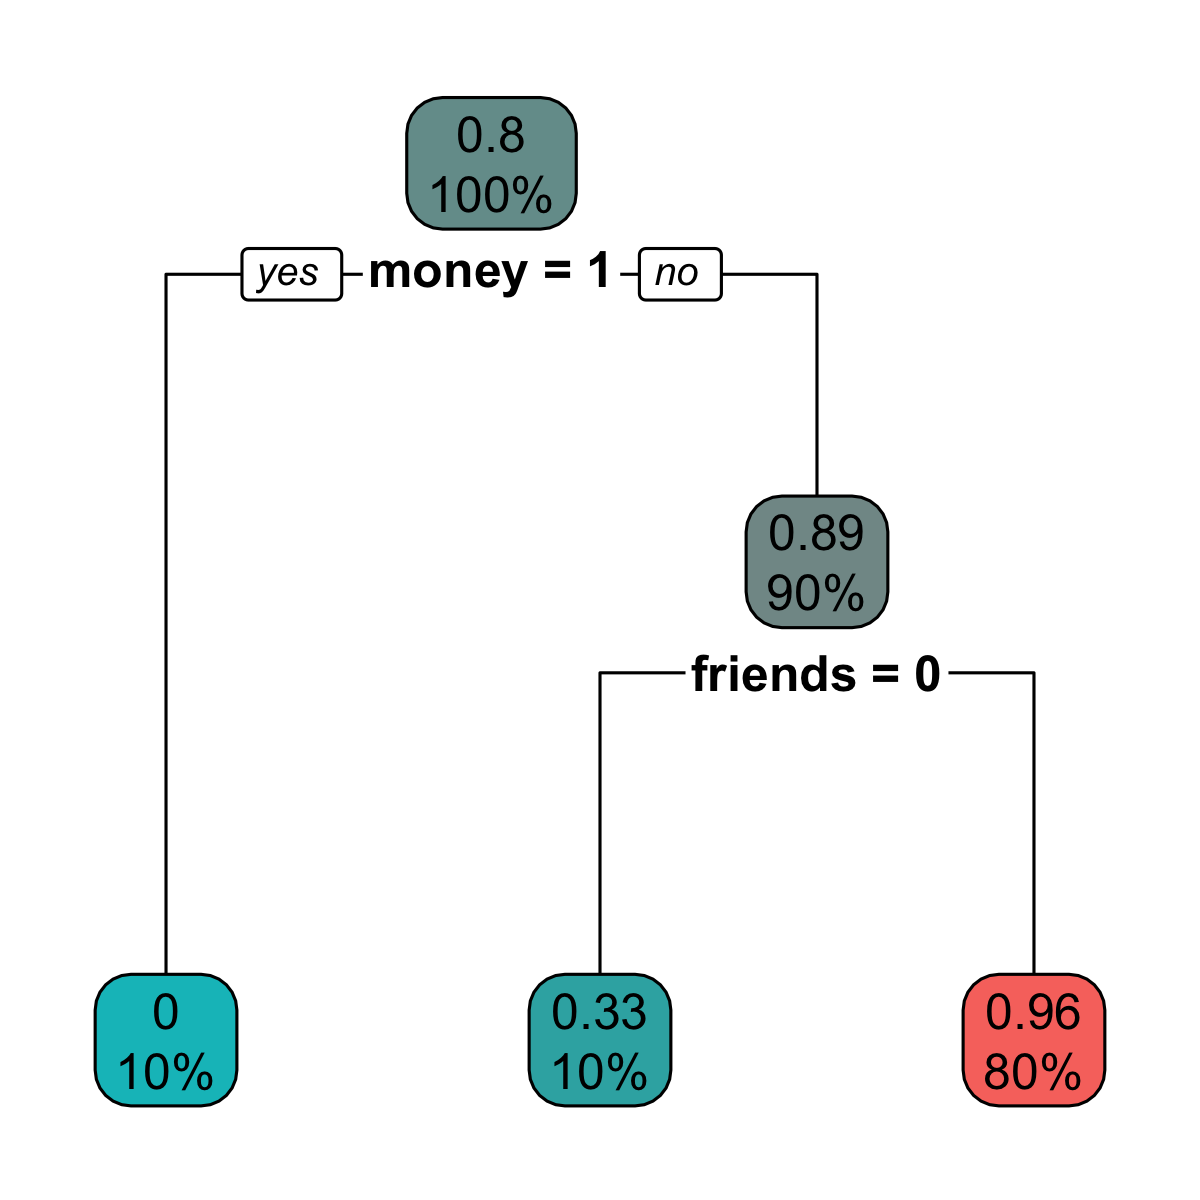
\includegraphics[width=0.6\textwidth]{img/happiness-boosting-tree-3.png}
\end{center}

Here are the predictions for this tree, along with the current weights.

{\small
\begin{center}
\begin{tabular}{cccc}
\toprule
Datapoint ID & $w_i^{(3)}$ & happy $(Y)$ & $G_3(x)$ \\
\midrule
1 & 0.1 & -1 & -1 \\
2 & 0.1 & -1 & -1 \\
3 & 0.1 & -1 & -1 \\
4 & 0.1 & -1 & -1 \\
5 & 0.1 & -1 & 1 \\
6 & 0.1 & -1 & -1 \\
\midrule
7 & 0.4 & 1 & 1 \\
8 & 0.4 & 1 & 1 \\
9 & 0.1 & 1 & -1 \\
10 & 1.5 & 1 & 1 \\
\bottomrule
\end{tabular}
\end{center}
}

\item[(i)] Compute the misclassification error of this tree, $\text{err}_3$. 

$$ \text{err}_3 = \qquad \qquad \qquad $$
\vspace{3mm}

\item[(j)] Based on how $G_3(x)$ performs, calculate $\alpha_3$, its voting weight.
$$ \alpha_3 = \qquad \qquad \qquad $$

\item[(k)] Re-weight the observation weights for the training examples. 
\begin{center}
\begin{tabular}{p{0.45\textwidth}p{0.45\textwidth}}
$w_1^{(4)} = $ \hfill & $w_6^{(4)} = $ \hfill \\
$w_2^{(4)} = $ \hfill & $w_7^{(4)} = $ \hfill \\
$w_3^{(4)} = $ \hfill & $w_8^{(4)} = $ \hfill \\
$w_4^{(4)} = $ \hfill & $w_9^{(4)} = $ \hfill \\
$w_5^{(4)} = $ \hfill & $w_{10}^{(4)} = $ \hfill \\
\end{tabular}
\end{center}

\item[(l)] Now we grow another decision tree, $G_4(x)$, using these new weights as inputs to the \texttt{rpart} package. 

\begin{center}
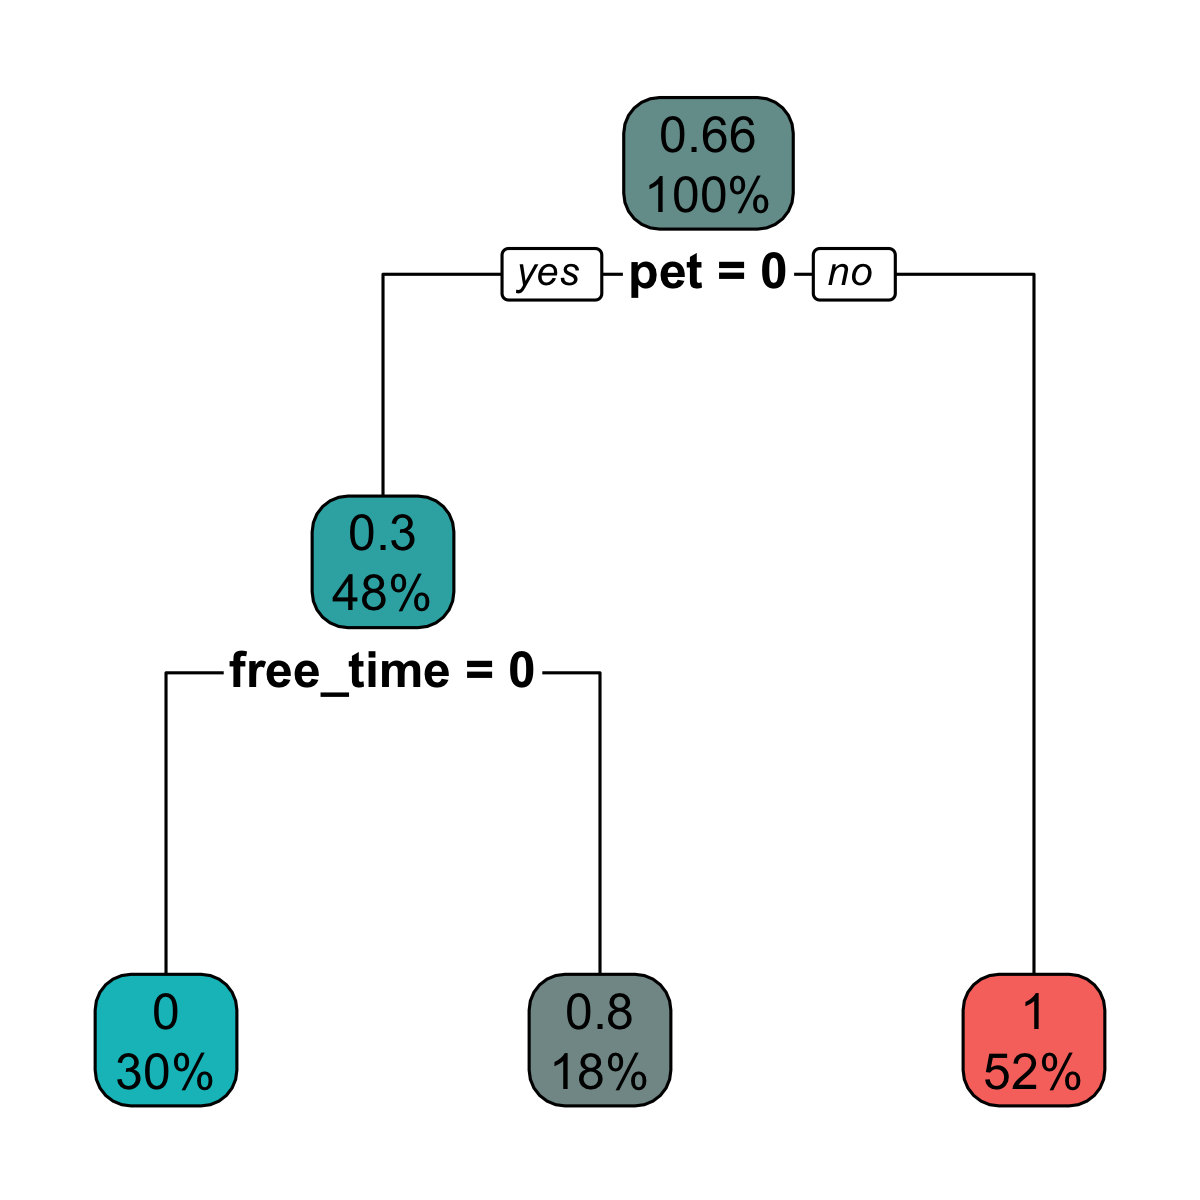
\includegraphics[width=0.6\textwidth]{img/happiness-boosting-tree-4.png}
\end{center}

Here are the predictions for this tree, along with the current weights.

{\small
\begin{center}
\begin{tabular}{cccc}
\toprule
Datapoint ID & $w_i^{(4)}$ & happy $(Y)$ & $G_4(x)$ \\
\midrule
1 & 0.1 & -1 & -1 \\
2 & 0.1 & -1 & -1 \\
3 & 0.1 & -1 & -1 \\
4 & 0.1 & -1 & -1 \\
5 & 1.4 & -1 & 1 \\
6 & 0.1 & -1 & -1 \\
\midrule
7 & 0.4 & 1 & 1 \\
8 & 0.4 & 1 & 1 \\
9 & 1.4 & 1 & 1 \\
10 & 1.5 & 1 & 1 \\
\bottomrule
\end{tabular}
\end{center}
}

\item[(m)] Compute the misclassification error of this tree, $\text{err}_4$. 

$$ \text{err}_4 = \qquad \qquad \qquad $$
\vspace{3mm}

\item[(n)] Based on how $G_4(x)$ performs, calculate $\alpha_4$, its voting weight.
$$ \alpha_4 = \qquad \qquad \qquad $$

\item[(o)] Output the weighted average of the four classifiers' votes for each training example:
$$ G(x) = \text{sign}\left[ \alpha_1 G_1(x) + \alpha_2 G_2(x) + \alpha_3 G_3(x) + \alpha_4 G_4(x) \right] $$ 
What is the final training error? 
\vspace{3mm}
{\small
\begin{center}
\begin{tabular}{cccccc|c}
\toprule
Datapoint ID & happy $(Y)$ & $G_1(x)$ & $G_2(x)$ & $G_3(x)$ & $G_4(x)$ & $G(x)$ \\
\midrule
1 & -1 & -1 & -1 & -1 & -1 & \\
2 & -1 & -1 & -1 & -1 & 1 & \\
3 & -1 & -1 & -1 & -1 & 1 & \\
4 & -1 & -1 & -1 & -1 & -1 & \\
5 & -1 & -1 & -1 & 1 & -1 & \\
6 & -1 & -1 & -1 & -1 & -1 & \\
\midrule
7 & 1 & -1 & 1 & 1 & 1 & \\
8 & 1 & -1 & 1 & 1 & 1 & \\
9 & 1 & 1 & 1 & -1 & 1 & \\
10 & 1 & 1 & -1 & 1 & 1 & \\
\bottomrule
\end{tabular}
\end{center}
}
\end{enumerate} 

\vspace{3mm}

\begin{question}{}
The most difficult thing to understand in all of this is how the updated weights play into the construction of subsequent trees. A clue comes from the dataset percentages shown in the nodes of each tree. For example, trees $1$ and $3$ actually have the same structure, but the impurities at each node are different due to the different weights. Discuss how the weights could inform the variables the splitting algorithm chooses to split on (revisit Chapter~\ref{chapter:decisiontrees}, if necessary, to see the math). 
\end{question}

\newpage

%%%%%%%%%%%%%%%%%%%%%%%%%%%%%%%%%%%%%%%%%%%%%%%%%%%%%%%%%%%%%%%%%%%%%%%%%%%%%%%%%%%%%%%%

\section{Revisiting Breast Cancer Classification}

Let's once again revisit the classification example for which we built a single decision tree in Chapter~\ref{chapter:decisiontrees} and a random forest in Chapter~\ref{chapter:randomforests}. The Wisconsin Breast Cancer Dataset contains information about $30$ different imaging features of fine needle aspirate (FNA) samples from breast masses in $569$ study participants.

Here is a plot showing the evolution of the training and test error as a function of the number of trees:
\begin{center}
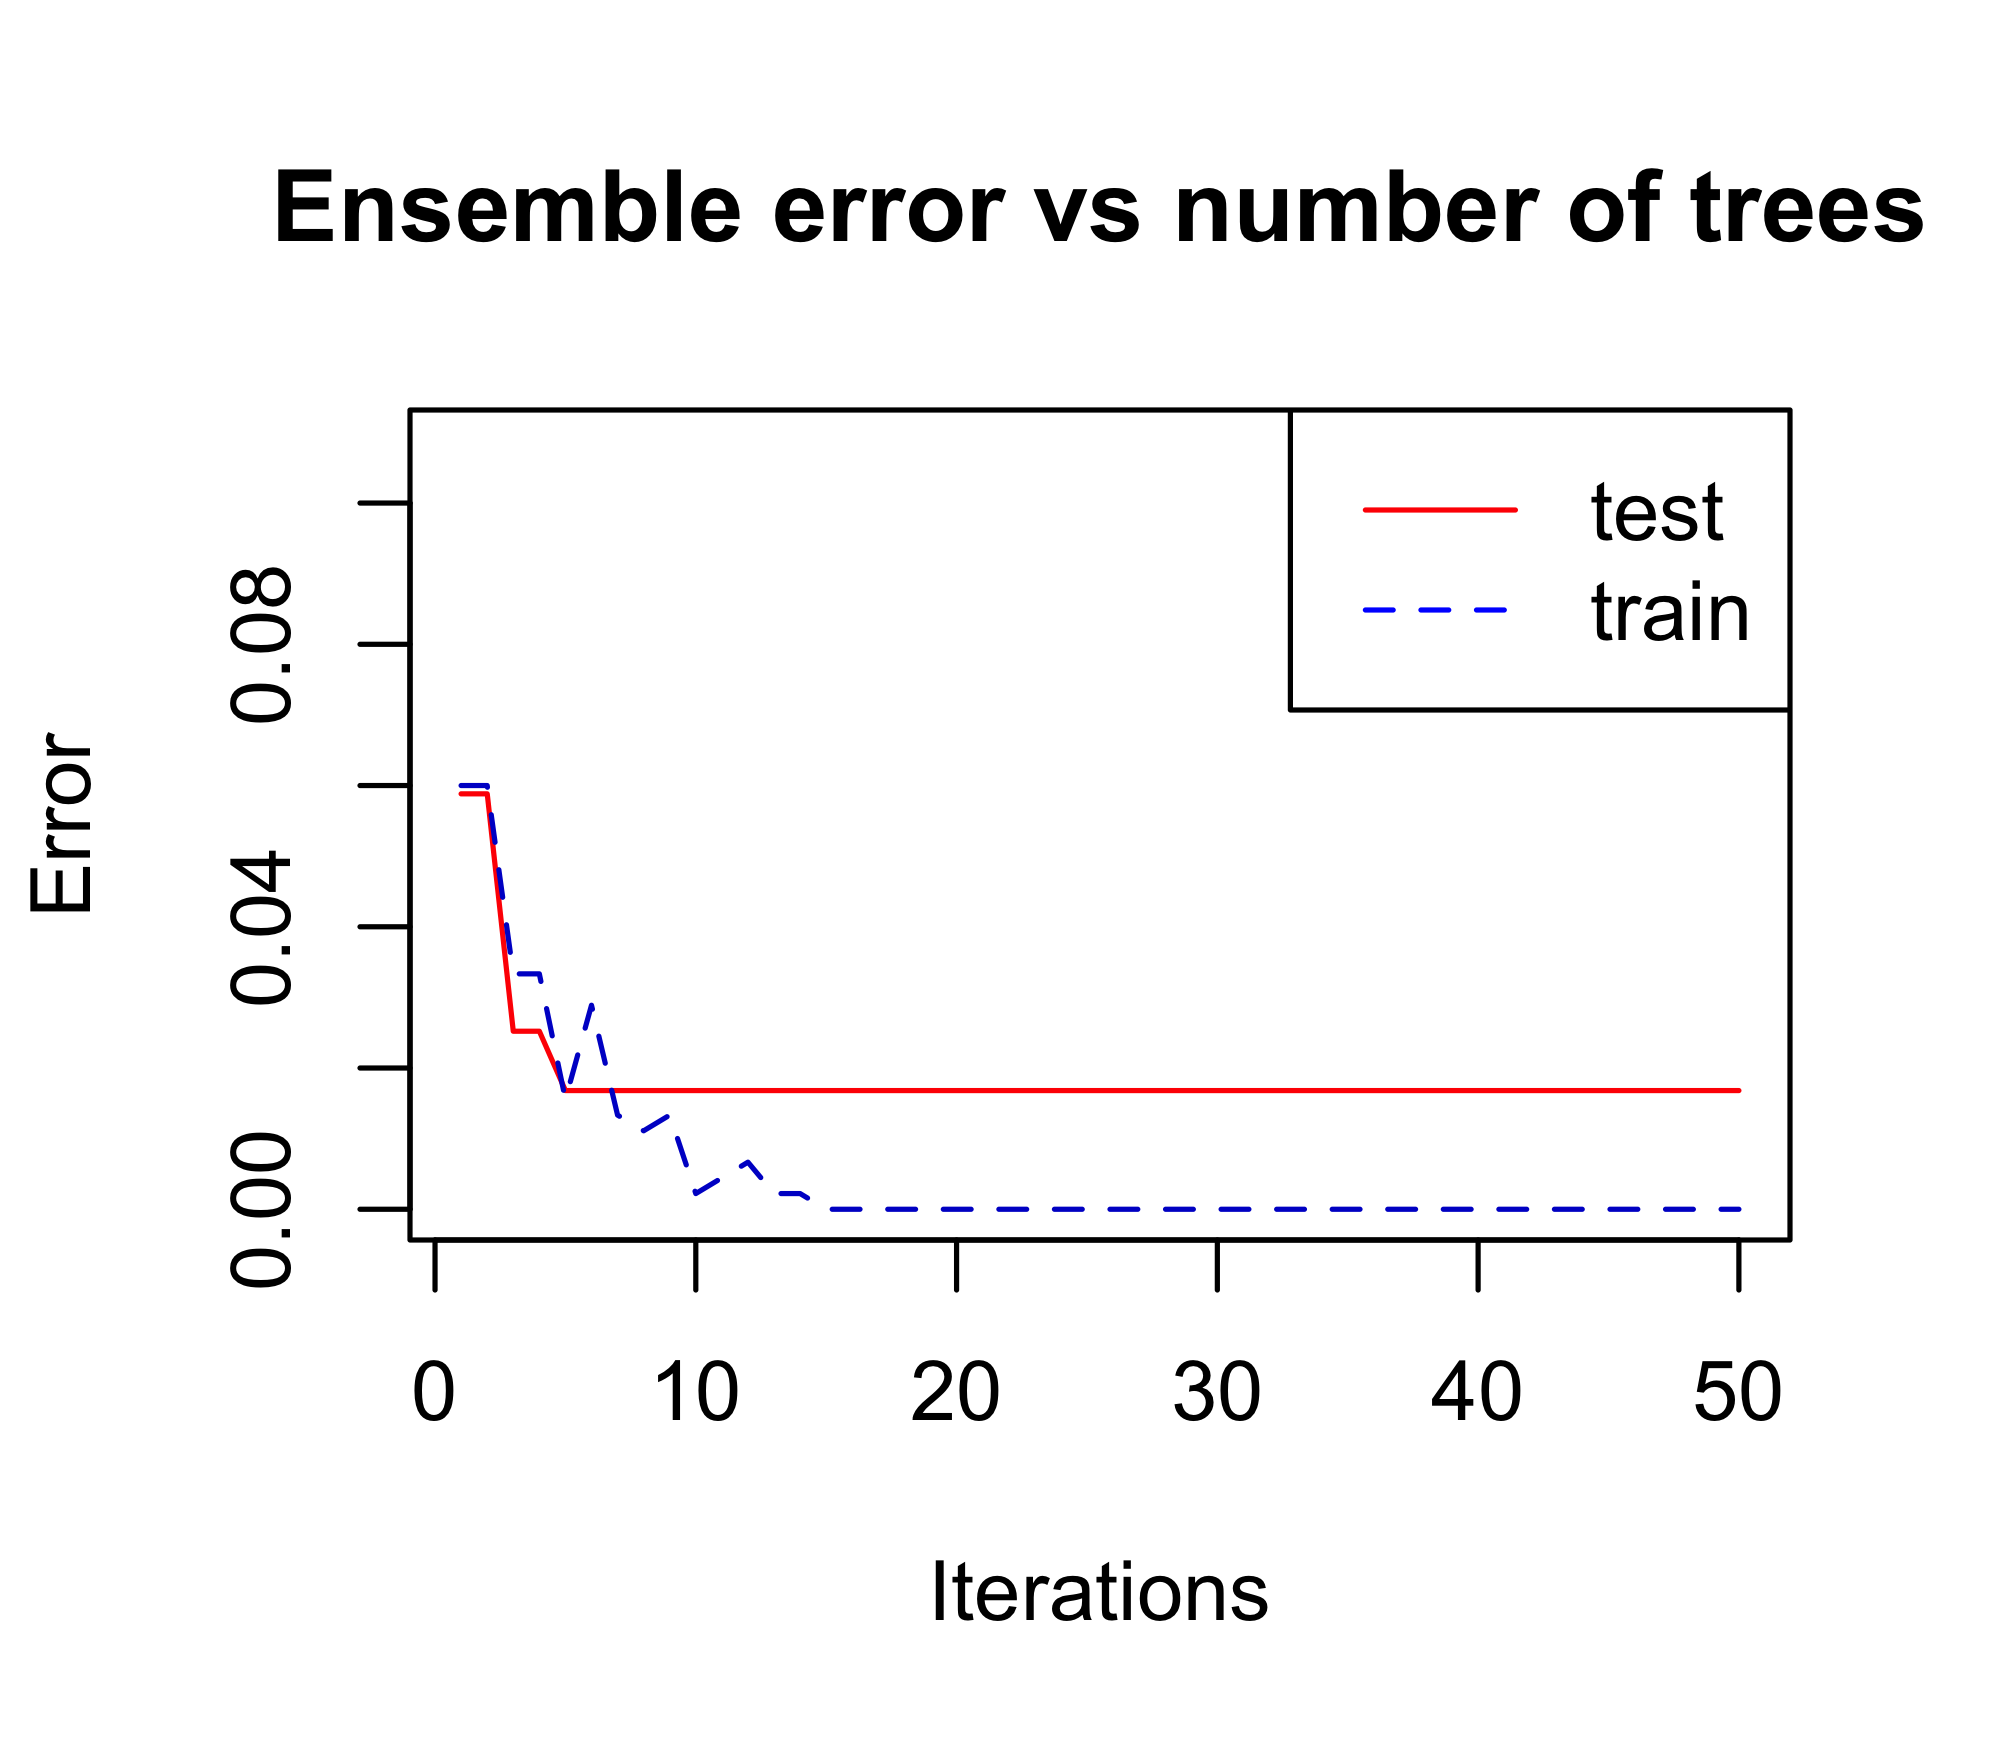
\includegraphics[width=0.7\textwidth]{img/wisconsin-boosting-error.png}
\end{center}
where $450$ samples are used for training and the remaining $119$ for testing. Here are tree numbers 1, 3, 6, and 8:
\begin{center}
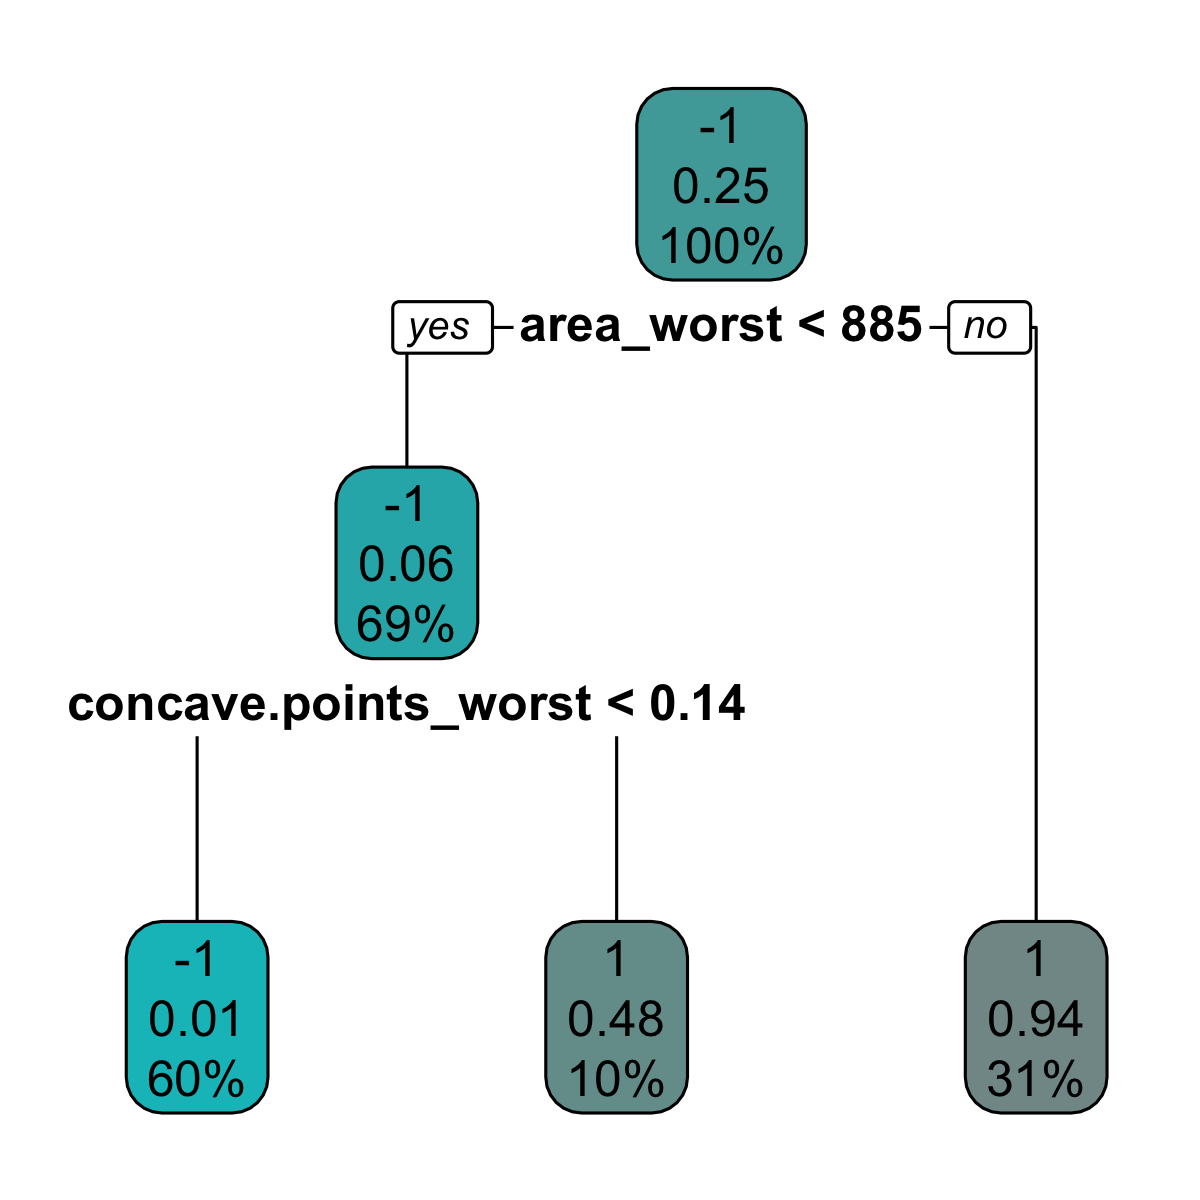
\includegraphics[width=0.45\textwidth]{img/wisconsin-boosting-tree-1.png}
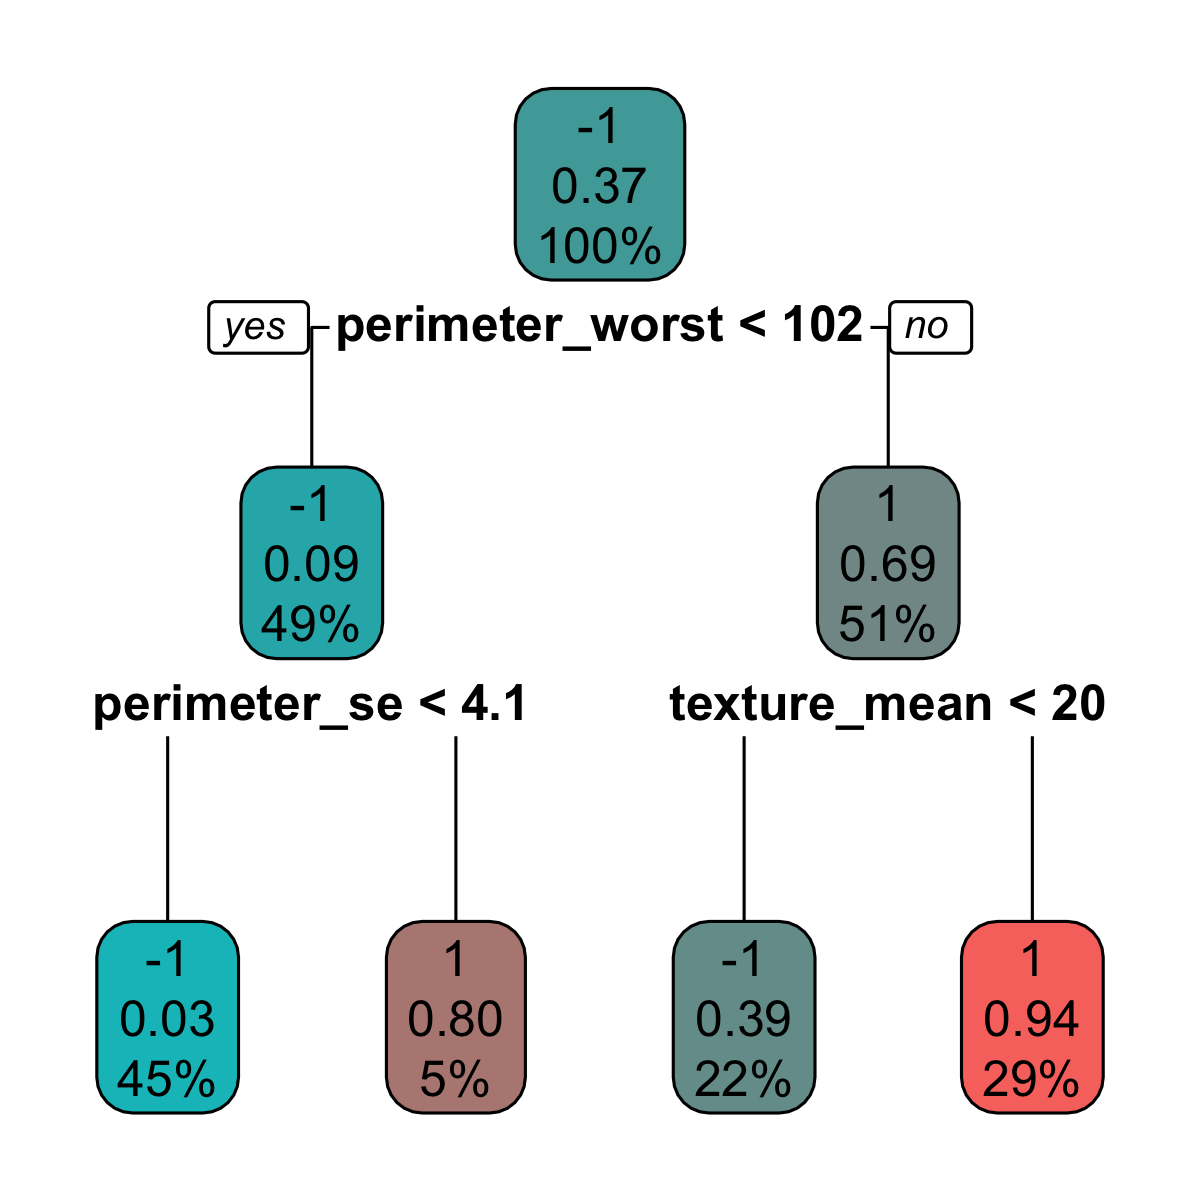
\includegraphics[width=0.45\textwidth]{img/wisconsin-boosting-tree-3.png}
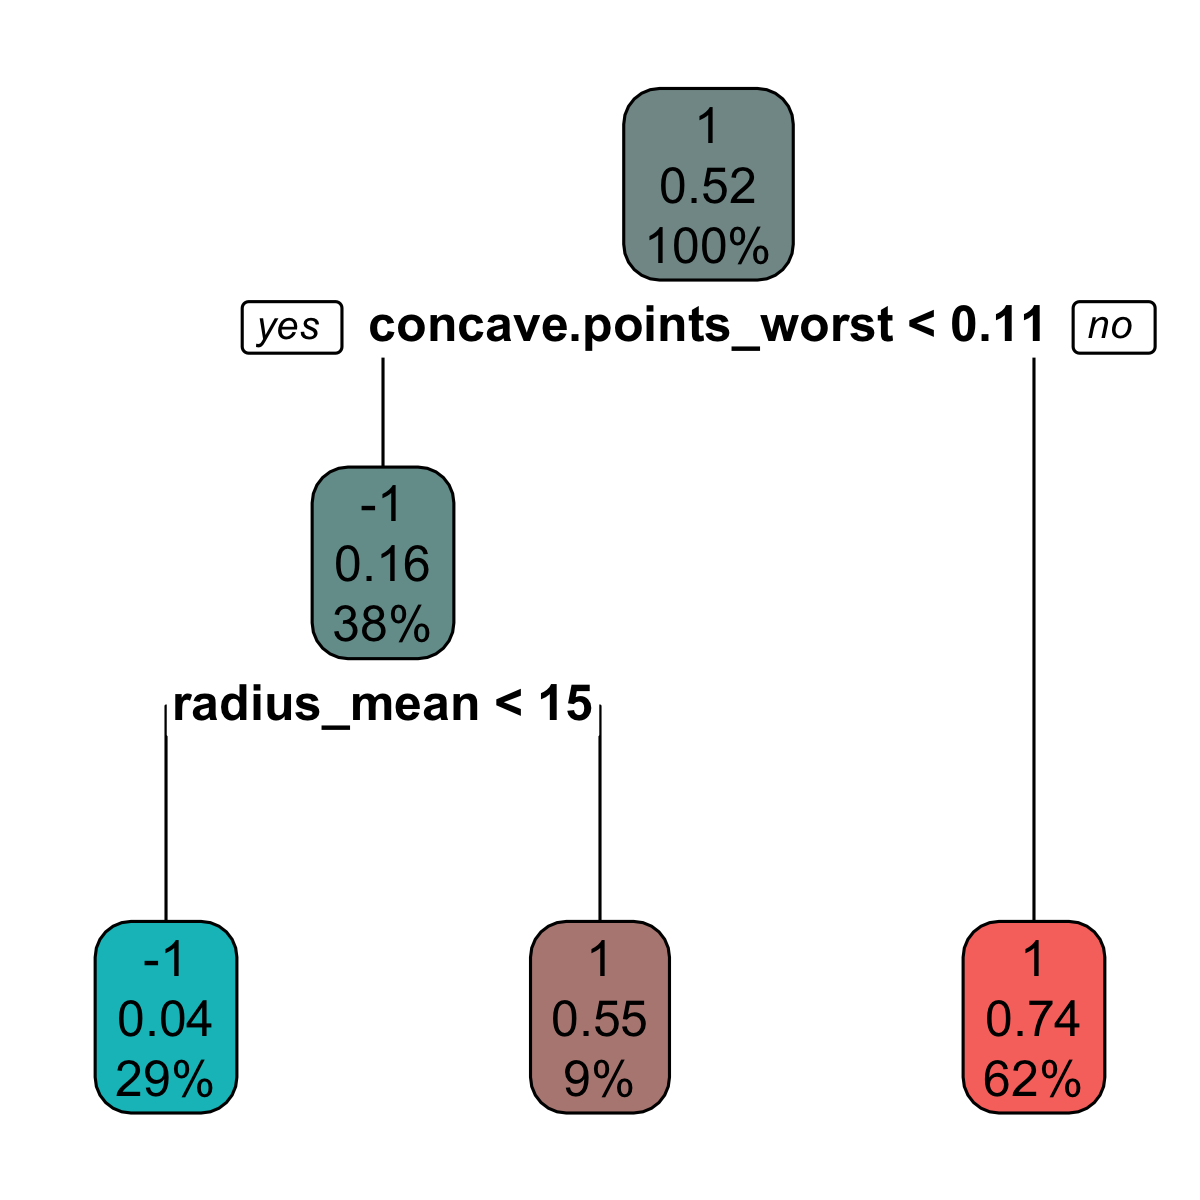
\includegraphics[width=0.45\textwidth]{img/wisconsin-boosting-tree-6.png}
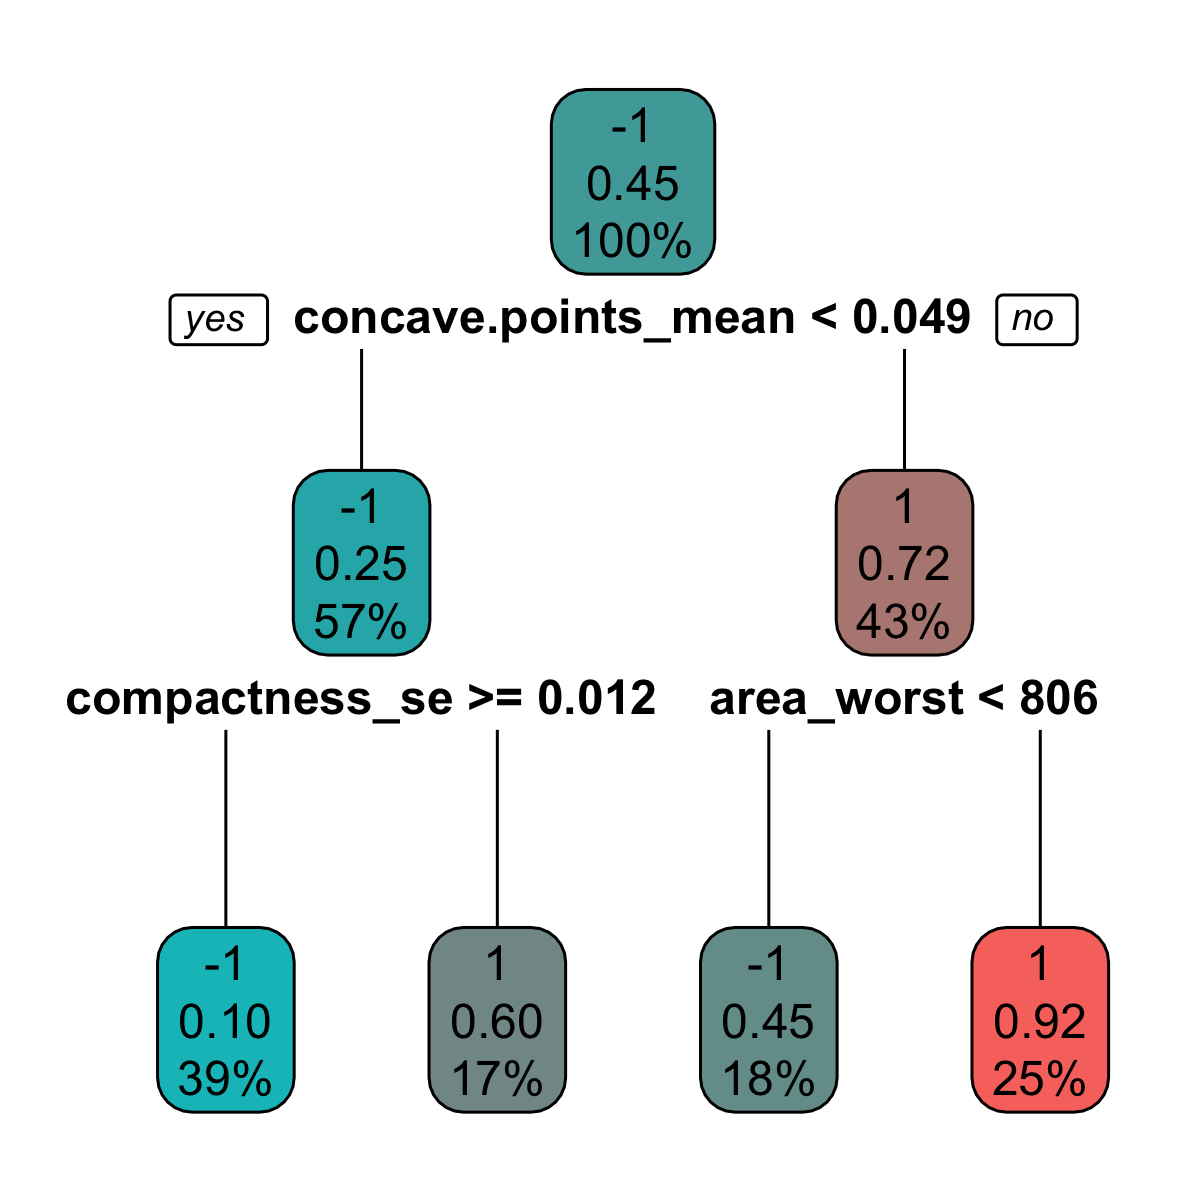
\includegraphics[width=0.45\textwidth]{img/wisconsin-boosting-tree-8.png}
\end{center}

\vspace{3mm}

\begin{question}{}
Compare and contrast boosting and random forests on the basis of:
\begin{itemize}
\item Whether each tree uses all or part of the dataset
\item Whether they consider a subset of the predictors at each split or all the predictors
\item Whether you can parallelize the construction of different trees (i.e., build them at the same time on different processors)
\item Whether the votes of different classifiers are independent
\item Ease of use and interpretability
\end{itemize}
\end{question}

